
\section{Project Management}
The following section outlines the processes undertaken during the various stages of the project’s planning and development. It also describes the manner in which decisions regarding design and implementation were conducted. 

\subsection{Brainstorming}
The first stage of the project involved an exploration of the latest advancements in the software development domain. In the search for a viable project idea, themes such as artificial intelligence, Internet of Things, virtual reality and augmented reality were investigated and considered. During this phase, both news and scholarly articles were reviewed to identify trends and growing areas pertinent to the computing field. Following that, a base of possible topics fitting the criteria for this Applied Project \& Minor dissertation was compiled. With the guidance of my supervisor, the topic that piqued the interest the was selected - AR. 

Following determining the area of interest, a period was spent establishing the state of the field in Augmented Reality. The primary method employed to grasp a sense of the possibilities available was reading and documenting the latest advancements relating to AR.


\subsection{Agile}
Given the changing nature of this research-heavy project, employing Agile methodologies was crucial to facilitate an effective development cycle.

Initially, a period was spent researching the most effective software development methodology. Given the changeability of a research-based project, a Waterfall model with meticulous planning was immediately ruled out. It was concluded an Agile Method would be most appropriate. Choosing which Agile methodology to employ provoked further research. Literature indicates that there is a lack of statistical evidence relating to whether a Scrum or Kanban approach is most effective\cite{sugimori1977toyota}. For this reason, a combination of Kanban and Scum methodologies were applied to implement Agile Development. Given it was just one developer working on this project, the luxury of creating a developer specific workflow was exercised. Various elements from the outlined Agile methodologies were combined, to create a custom project planning and software development method.

\subsubsection{Kanban}
The Kanban methodology was implemented throughout the project development. To facilitate the creation and management of storyboards, Trello was used. A board was created with three stages - \say{To Do}, \say{In Progress}, \say{Done}. Tasks representing the project’s critical path were added as cards via Trello’s user interface.

\begin{figure}[!ht]
\caption{Trello Storyboard}
\centering
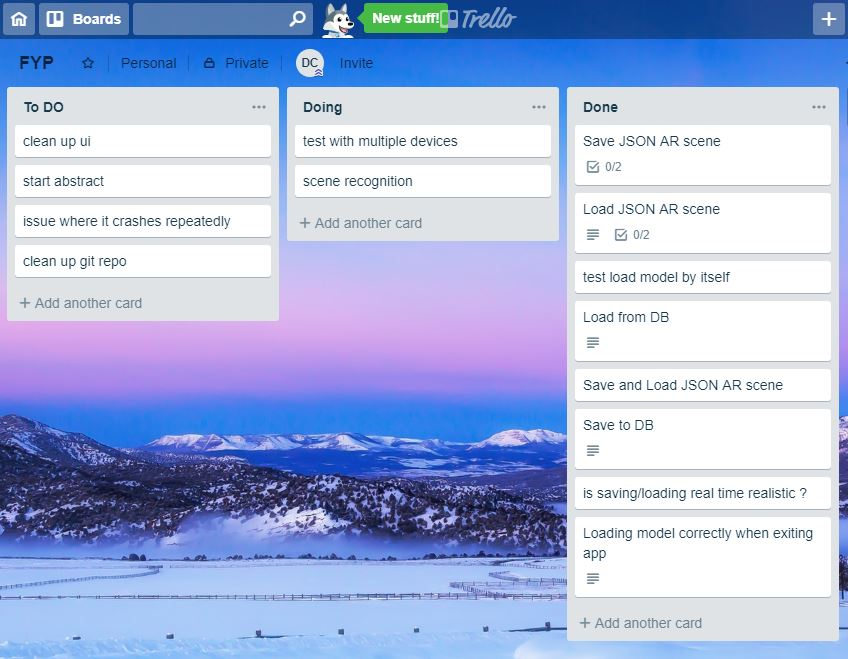
\includegraphics[width=1\textwidth]{images/trello.JPG}
\end{figure}

\subsubsection{SCRUM}
In conjunction with Kanban, the Scrum methodology was executed. In this project, sprints were one week in length. At the end of each week, a meeting took place between developer and supervisor. During this time progress from the sprint was discussed along with any ‘blockers’(hindrances to project development). Goals for the next sprint were also established and logged in the GitHub readme following these meetings. 


\section{Version Control}
\subsection{Github}
Github was used as the method of version control in this project. A remote Git repository was created on Github. During development, code was tracked using git and then uploaded to this repo. Github provided two primary functions for development, tracking code changes and also the security of having the code base backed up in case of any issues on my local machine. Sprint planning was also logged on the github readme.  


\section{Literature Review}
To gather relevant literature sources, science and computing databases (ScienceDirect, Omni File Full, Mega text, Science Citation Index) were queried. To gather information pertaining to AR technologies, databases were queried for the strings ”augmented reality” AND ”state of the field” OR ”state of the art”. To find resources relating to augmented reality in the context of architecture, the strings ”augmented reality” AND ”architecture” OR ”architectural” were queried. Previous literature [3], highlights that there is a lack of consistency in both academic and professional fields when discussing augmented reality as it is often used interchangeably with other mixed reality technologies. To combat this, the NOT operator was used on the term ”virtual reality” as this review solely examines the application of augmented reality technologies. In cases specific to outlining current technologies, such as software development toolkits, developer documentation from internet sources are referenced.

The topic was expanded upon by researching databases for articles and publications on the topic. However, given that the area itself is considered ‘bleeding edge’, informative resources proved scarce. It was found to be more effective to investigate documentation relating to current AR SDKs and review whether they featured the required functionality to implement shared AR. This documentation was also used to understand the various processes behind building collaborative AR experiences.  While this stage initially presented itself as quite challenging due to the limited resources available relating to the topic, it manifested as an exciting opportunity to make a contribution to shared AR’s limited body of research.

\section{Testing}
\subsection{Web Application Testing}
Selenium was chosen as the method of testing the system's web application. Having had previous experience with the Selenium IDE, it was for this reason it was selected as a testing method.
\subsection{Augmented Reality Testing}
Sourcing a method of testing the augmented reality aspect of mobile application proved challenging at first. However, it was eventually decided that testing the robustness of the application's plane detection and tracking would be beneficial. This was achieved by attempting to place an AR trackable in a selection of contrasting lighting conditions and evaluating the effectiveness and speed of the plane detection. 




\section{System Architecture}
The system is comprised of three primary components:
\begin{itemize}
    \item Ionic AR Mobile application
    \item Firebase NO-SQL database
    \item Ionic Web Application
\end{itemize}


\begin{figure}[!ht]
\caption{System Architecture}
\centering
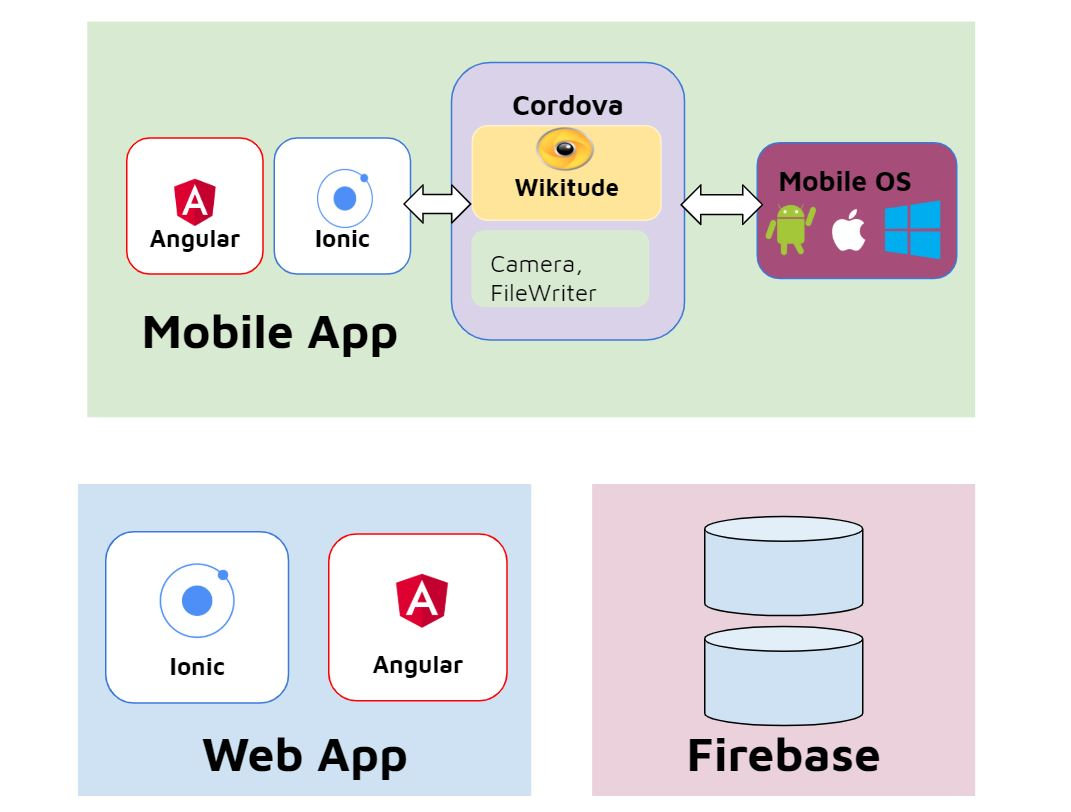
\includegraphics[scale=0.5]{images/sys_architecture.JPG}
\end{figure}


\subsection{Ionic Framework}
In conjunction with Apache Cordova, the mobile application was built using Ionic 3. Ionic was selected because it supports the creation of cross-platform applications through the use of web technologies. Additionally, it integrates with Apache Cordova, which includes a plugin for the Wikitude SDK. Ionic handles the front-end side of this application, i.e the components that comprise the User Interface, while Apache Cordova provides plugins and support or access to the hardware of the native device. 

\subsection{Wikitude Cordova plugin}
The Wikitude Apache Cordova plugin was used to add Wikitude’s functionality to the mobile application. To include it in the project, the following command was executed using the ionic CLI tool. 
\begin{minted}
[
baselinestretch=1.2,
fontsize=\footnotesize,
linenos
]
{java}
ionic cordova plugin add https://github.com/Wikitude/wikitude-cordova-plugin.git

\end{minted}


\subsection{Firebase}
Firebase was chosen as the database for the project because of its support for applications built using web technologies. NPM was used to install the firebase plugin.

\begin{minted}
[
baselinestretch=1.2,
fontsize=\footnotesize,
linenos
]
{java}
npm install --save firebase
\end{minted}



An API key is required to use firebase. This was obtained by accessing the Firebase Console via the Google Cloud Platform. With the application registered and configured, the firebase credentials were then added to the Ionic Application in the firebase.credentails.ts file.

Firebase’s real-time database is used to facilitate Shared AR within the application. A reference to the database was created within the application. Following this, a listener was added to the database reference. This allows the application to be automatically notified of any changes to the database. 

\begin{minted}
[
baselinestretch=1.2,
fontsize=\footnotesize,
linenos
]
{javascript}
// create databse refernce
        var ref = firebase.database().ref('/ARSessions/');

             // getting the latest data from the db
              this.ref.on('value', snapshot => {
                dbres = snapshot.val();
              });

\end{minted}

In the context of this mobile application and shared AR, this functionality is used to update the user’s AR scene in real time in the event of changes made to it by another user. In this manner, all users are in sync - viewing and interacting with the same ar scene loaded via the same database reference.
